\documentclass{article}
\usepackage{ctex}
\usepackage{amsmath}
\usepackage{graphicx}
\usepackage{wrapfig}
\usepackage{caption}
\usepackage[top=0.8in, bottom=0.8in,left=0.8in, right=0.8in]{geometry}
\usepackage{float} 
\usepackage{subfigure}
\usepackage{subcaption}
\usepackage{bm}
\xeCJKsetup{CJKmath=true} 

\begin{document}
\section*{可爱的杆(60分)}
\begin{wrapfigure}{r}{7cm}
	\vspace{-15pt}    % 对应高度1
	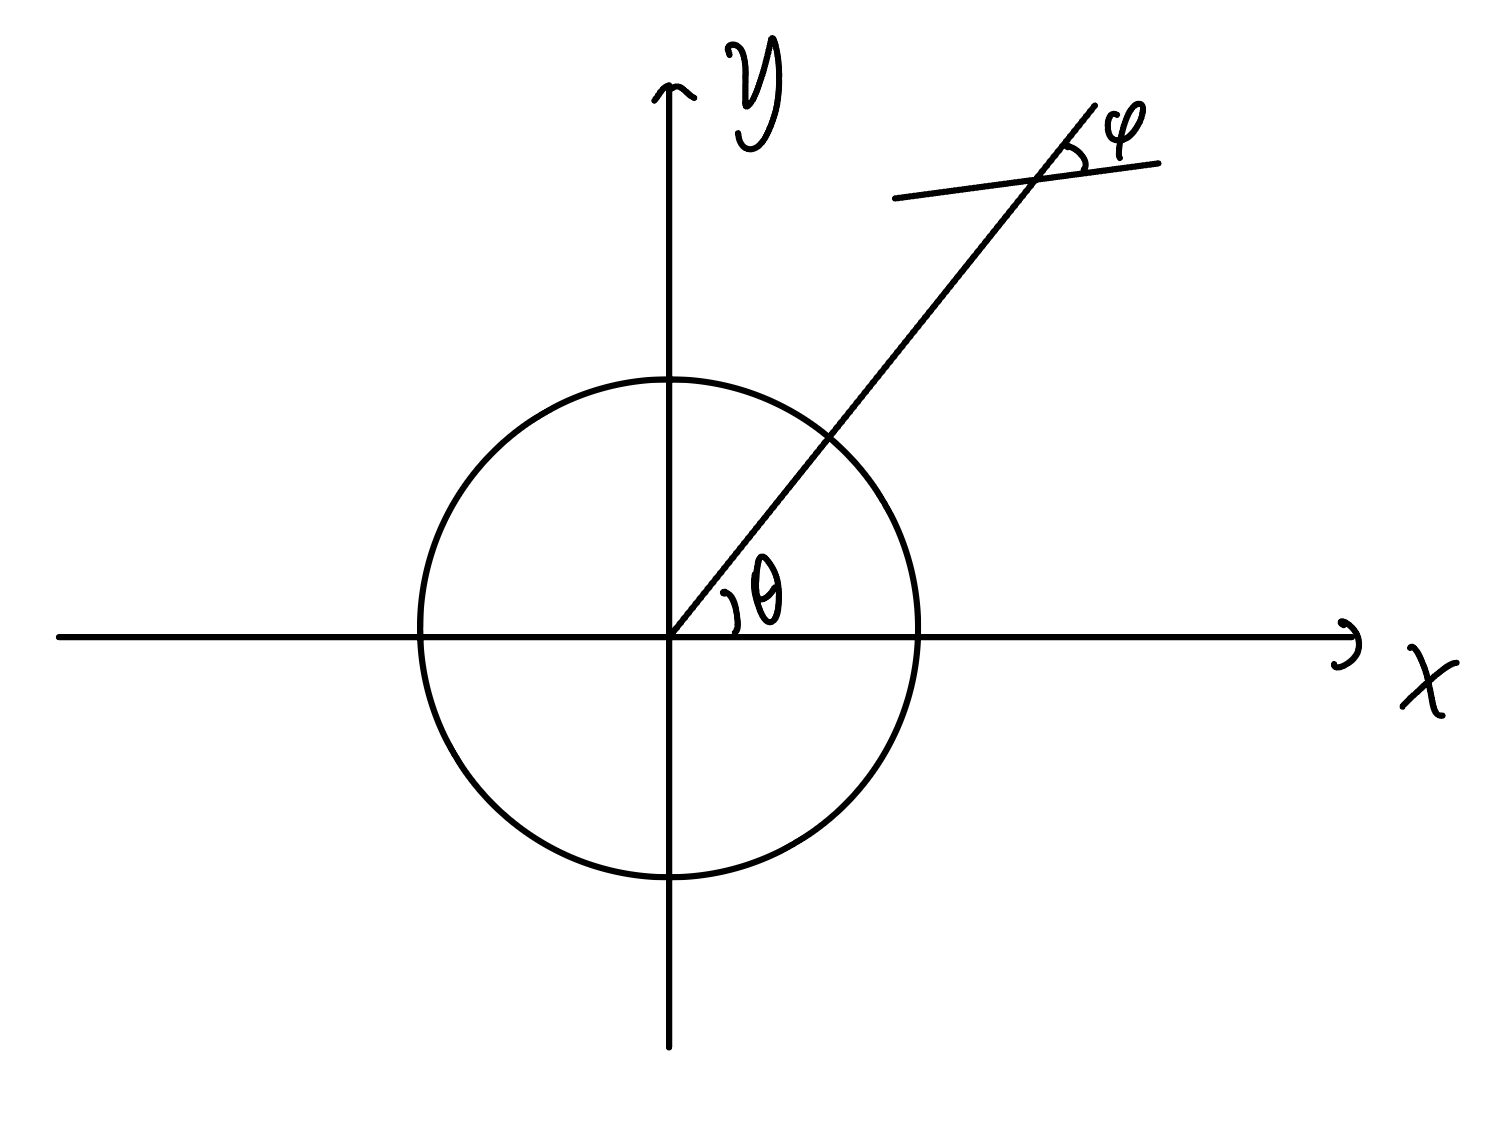
\includegraphics[width=7cm]{img/0010.1.jpeg}\\
	\vspace{-15pt}    % 对应高度2
	\caption{}
	\vspace{-15pt}    % 对应高度3
\end{wrapfigure}
一根杆位于太空中绕一质量为$M$的中心天体旋转。杆质地坚硬,长为$2l$,质量为$m$,杆质心距离中心天体$r$,角度$\varphi$如图所示,已知$r\gg l$
\begin{itemize}
\item[(1)]求使$r,\dot{\theta},\varphi$不随时间变化的\textbf{稳定的}$\varphi$值。并求出此时$r,\dot{\theta}$应满足的关系,保留至 $\frac{l^2}{r^2}$阶。
\item[(2)]
\begin{itemize}
    \item[(i)]设系统原来以(1)中稳定的运动方式运动,现给杆微扰,使其具有一定的$\dot{r},\dot{\varphi}$初始值,试求有关$r,\theta,\varphi$的运动微分方程
    \item[(ii)]令$r=r_0+\Delta r$,$\dot{\theta}=\omega_0+\Delta \omega$,其中满足$\dfrac{\Delta r}{r_0}\ \~{}\ \dfrac{\Delta \omega}{\omega_0} \ \~{}\ \varphi\ \~{}\ \dfrac{l^2}{l_0^2}\ll 1$,试求$\varphi$具有的两种频率(不必求出特解),并判断两频率是否与$l$相关。试就两频率的来源分别简述原因
    \item[(iii)]  求此时杆质心运动的旋进角速度。(原运动完成一个周期后,矢径转过的角度与原运动得到周期比值)
\end{itemize} 
\end{itemize}
\end{document} 